\section{DIL\_\-entry  Class Reference}
\label{classDIL__entry}\index{DIL_entry@{DIL\_\-entry}}
{\tt \#include $<$dil2al.hh$>$}

Inheritance diagram for DIL\_\-entry::\begin{figure}[H]
\begin{center}
\leavevmode
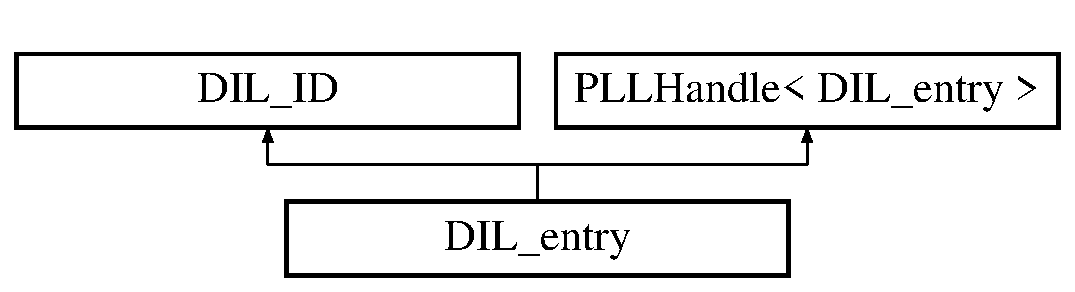
\includegraphics[height=2cm]{classDIL__entry}
\end{center}
\end{figure}
\subsection*{Public Methods}
\begin{CompactItemize}
\item 
{\bf DIL\_\-entry} ({\bf Text\_\-File\_\-Buffers} \&t)
\item 
{\bf DIL\_\-entry} ({\bf Text\_\-File\_\-Buffers} \&t, {\bf String} \&idstr)
\item 
{\bf DIL\_\-entry} ({\bf Text\_\-File\_\-Buffers} \&t, const {\bf Sub\-String} \&idstr)
\item 
{\bf $\sim$DIL\_\-entry} ()
\item 
DIL\_\-entry $\ast$ {\bf elbyid} (const {\bf DIL\_\-ID} \&id) const
\item 
DIL\_\-entry $\ast$ {\bf operator[$\,$]} ({\bf DIL\_\-ID} \&id)
\item 
{\bf DIL\_\-Topical\_\-List} $\ast$ {\bf Topics} (int n)
\item 
{\bf DIL\_\-AL\_\-List} $\ast$ {\bf Projects} (int n)
\item 
void {\bf Set\_\-Semaphore} (int svalue)
\item 
int {\bf Get\_\-Semaphore} ()
\item 
void {\bf Set\_\-Semaphores} (int svalue)
\item 
time\_\-t {\bf Propagated\_\-Target\_\-Date} (bool warn, bool top={\bf true}) const
\item 
time\_\-t {\bf Target\_\-Date} (bool top={\bf true}) const
\item 
time\_\-t {\bf Local\_\-Target\_\-Date} (int n, time\_\-t unspecified=-2)
\item 
time\_\-t {\bf Time\_\-Required} ()
\item 
float {\bf Completion\_\-State} ()
\item 
{\bf String} $\ast$ {\bf Entry\_\-Text} ()
\item 
bool {\bf Get\_\-Entry\_\-Parameters} ({\bf String} \&parstr)
\item 
bool {\bf Is\_\-Direct\_\-Dependency\_\-Of} (const DIL\_\-entry $\ast$superior)
\item 
bool {\bf Is\_\-Dependency\_\-Of} (DIL\_\-entry $\ast$superior)
\item 
bool {\bf Has\_\-Superiors} (bool taggedonly={\bf false})
\item 
int {\bf Is\_\-Plan\_\-Entry} ()
\item 
bool {\bf Write\_\-to\_\-Binary\_\-Cache} (ofstream \&cfl)
\item 
bool {\bf Write\_\-Topical\_\-to\_\-Binary\_\-Cache} (ofstream \&cfl, bool gottext)
\item 
bool {\bf Read\_\-from\_\-Binary\_\-Cache} (ifstream \&cfl)
\item 
bool {\bf Read\_\-Topical\_\-from\_\-Binary\_\-Cache} (ifstream \&cfl, bool gottext)
\item 
bool {\bf Binary\_\-Cache\_\-Diagnostic} (DIL\_\-entry $\ast$cached, int \&testedbytes)
\end{CompactItemize}
\subsection*{Public Attributes}
\begin{CompactItemize}
\item 
{\bf DIL\_\-entry\_\-content} $\ast$ {\bf content}
\item 
{\bf DIL\_\-entry\_\-parameters} $\ast$ {\bf parameters}
\end{CompactItemize}
\subsection*{Protected Attributes}
\begin{CompactItemize}
\item 
int {\bf semaphore}
\item 
{\bf Text\_\-File\_\-Buffers} $\ast$ {\bf tfb}
\end{CompactItemize}


\subsection{Constructor \& Destructor Documentation}
\index{DIL_entry@{DIL\_\-entry}!DIL_entry@{DIL\_\-entry}}
\index{DIL_entry@{DIL\_\-entry}!DIL_entry@{DIL\_\-entry}}
\subsubsection{\setlength{\rightskip}{0pt plus 5cm}DIL\_\-entry::DIL\_\-entry ({\bf Text\_\-File\_\-Buffers} \& {\em t})}\label{classDIL__entry_a0}




Definition at line 913 of file utilities.cc.

Referenced by Propagated\_\-Target\_\-Date().



\footnotesize\begin{verbatim}913 : tfb(&t), DIL_ID(), content(NULL), parameters(NULL) {}
\end{verbatim}\normalsize 
\index{DIL_entry@{DIL\_\-entry}!DIL_entry@{DIL\_\-entry}}
\index{DIL_entry@{DIL\_\-entry}!DIL_entry@{DIL\_\-entry}}
\subsubsection{\setlength{\rightskip}{0pt plus 5cm}DIL\_\-entry::DIL\_\-entry ({\bf Text\_\-File\_\-Buffers} \& {\em t}, {\bf String} \& {\em idstr})}\label{classDIL__entry_a1}




Definition at line 915 of file utilities.cc.



\footnotesize\begin{verbatim}915 : tfb(&t), DIL_ID(idstr), content(NULL), parameters(NULL) {}
\end{verbatim}\normalsize 
\index{DIL_entry@{DIL\_\-entry}!DIL_entry@{DIL\_\-entry}}
\index{DIL_entry@{DIL\_\-entry}!DIL_entry@{DIL\_\-entry}}
\subsubsection{\setlength{\rightskip}{0pt plus 5cm}DIL\_\-entry::DIL\_\-entry ({\bf Text\_\-File\_\-Buffers} \& {\em t}, const {\bf Sub\-String} \& {\em idstr})}\label{classDIL__entry_a2}




Definition at line 917 of file utilities.cc.



\footnotesize\begin{verbatim}917 : tfb(&t), DIL_ID(idstr), content(NULL), parameters(NULL) {}
\end{verbatim}\normalsize 
\index{DIL_entry@{DIL\_\-entry}!~DIL_entry@{$\sim$DIL\_\-entry}}
\index{~DIL_entry@{$\sim$DIL\_\-entry}!DIL_entry@{DIL\_\-entry}}
\subsubsection{\setlength{\rightskip}{0pt plus 5cm}DIL\_\-entry::$\sim$DIL\_\-entry ()\hspace{0.3cm}{\tt  [inline]}}\label{classDIL__entry_a3}




Definition at line 660 of file dil2al.hh.

References content, and parameters.



\footnotesize\begin{verbatim}660 { delete content; delete parameters; }
\end{verbatim}\normalsize 


\subsection{Member Function Documentation}
\index{DIL_entry@{DIL\_\-entry}!Binary_Cache_Diagnostic@{Binary\_\-Cache\_\-Diagnostic}}
\index{Binary_Cache_Diagnostic@{Binary\_\-Cache\_\-Diagnostic}!DIL_entry@{DIL\_\-entry}}
\subsubsection{\setlength{\rightskip}{0pt plus 5cm}bool DIL\_\-entry::Binary\_\-Cache\_\-Diagnostic (DIL\_\-entry $\ast$ {\em cached}, int \& {\em testedbytes})}\label{classDIL__entry_a26}




Definition at line 1108 of file utilities.cc.

References DIL\_\-entry\_\-parameters::Binary\_\-Cache\_\-Diagnostic(), DIL\_\-entry\_\-content::Binary\_\-Cache\_\-Diagnostic(), content, parameters, and VOUT.

Referenced by Detailed\_\-Items\_\-List::Binary\_\-Cache\_\-Diagnostic().



\footnotesize\begin{verbatim}1108                                                                              {
1109   // test if the quick load cache process works reliably
1110   // this is the original entry, cached is the one retrieved from the binary cache
1111   //   start of this object test
1112   int localtestedbytes = 0;
1113   if ((*this)!=(*cached)) VOUT << "*** DIL_ID mismatch\n"; // testing if DIL_ID==DIL_ID
1114   localtestedbytes += sizeof(DIL_ID) + sizeof(PLLHandle<DIL_entry>) + sizeof(semaphore) + sizeof(tfb) + sizeof(content) + sizeof(parameters);
1115   //   end of this object test
1116   if (localtestedbytes!=sizeof(DIL_entry)) VOUT << "*** testedbytes!=sizeof(DIL_entry)\n";
1117   if (content) {
1118     if (cached->content) {
1119       if (!content->Binary_Cache_Diagnostic(cached->content,testedbytes)) return false;
1120     } else VOUT << "*** entry has content, cached does not\n";
1121   } else if (cached->content) VOUT << "*** entry has no content, cached does\n";
1122   if (parameters) {
1123     if (cached->parameters) {
1124       if (!parameters->Binary_Cache_Diagnostic(cached->parameters,testedbytes)) return false;
1125     } else VOUT << "*** entry has parameters, cached does not\n";
1126   } else if (cached->parameters) VOUT << "*** entry has no parameters, cached does\n";
1127   testedbytes += localtestedbytes;
1128   return true;
1129 }
\end{verbatim}\normalsize 
\index{DIL_entry@{DIL\_\-entry}!Completion_State@{Completion\_\-State}}
\index{Completion_State@{Completion\_\-State}!DIL_entry@{DIL\_\-entry}}
\subsubsection{\setlength{\rightskip}{0pt plus 5cm}float DIL\_\-entry::Completion\_\-State ()\hspace{0.3cm}{\tt  [inline]}}\label{classDIL__entry_a15}




Definition at line 683 of file dil2al.hh.

References DIL\_\-entry\_\-content::completion.

Referenced by DIL\_\-Required\_\-Task\_\-Chunks().



\footnotesize\begin{verbatim}683 { if (content) return content->completion; return (float) 0.0; }
\end{verbatim}\normalsize 
\index{DIL_entry@{DIL\_\-entry}!elbyid@{elbyid}}
\index{elbyid@{elbyid}!DIL_entry@{DIL\_\-entry}}
\subsubsection{\setlength{\rightskip}{0pt plus 5cm}DIL\_\-entry $\ast$ DIL\_\-entry::elbyid (const {\bf DIL\_\-ID} \& {\em id}) const}\label{classDIL__entry_a4}




Definition at line 919 of file utilities.cc.

References PLLHandle$<$ DIL\_\-entry $>$::Next(), and PLLHandle$<$ DIL\_\-entry $>$::Prev().

Referenced by Plan\_\-entry\_\-content::Decision\_\-Ptr(), generate\_\-modify\_\-element\_\-FORM\_\-interface(), generate\_\-modify\_\-element\_\-FORM\_\-interface\_\-DIL\_\-entry\_\-parameters(), Detailed\_\-Items\_\-List::Get\_\-All\_\-Topical\_\-DIL\_\-Parameters(), modify\_\-DIL\_\-entry\_\-target\_\-date(), modify\_\-DIL\_\-group\_\-target\_\-dates(), modify\_\-element\_\-through\_\-FORM\_\-interface(), operator[$\,$](), Propagated\_\-Target\_\-Date(), Detailed\_\-Items\_\-List::Read\_\-Topical\_\-from\_\-Binary\_\-Cache(), DIL\_\-AL\_\-List::Superiorbyid(), Tabbed\_\-DIL\_\-Hierarchy(), Tabbed\_\-FORM\_\-DIL\_\-Hierarchy(), Tabbed\_\-HTML\_\-DIL\_\-Hierarchy(), and update\_\-DIL\_\-entry\_\-parameter\_\-elements().



\footnotesize\begin{verbatim}919                                                      {
920 // return pointer to list element with DIL ID id
921 //      if ((*const_cast<DIL_entry *>(this))==id) return const_cast<DIL_entry *>(this);
922         if ((*this)==id) return const_cast<DIL_entry *>(this);
923         for (DIL_entry * de=Next(); de; de=de->Next()) if (*de==id) return de;
924         for (DIL_entry * de=Prev(); de; de=de->Prev()) if (*de==id) return de;
925         return NULL;
926 }
\end{verbatim}\normalsize 
\index{DIL_entry@{DIL\_\-entry}!Entry_Text@{Entry\_\-Text}}
\index{Entry_Text@{Entry\_\-Text}!DIL_entry@{DIL\_\-entry}}
\subsubsection{\setlength{\rightskip}{0pt plus 5cm}{\bf String}$\ast$ DIL\_\-entry::Entry\_\-Text ()\hspace{0.3cm}{\tt  [inline]}}\label{classDIL__entry_a16}




Definition at line 684 of file dil2al.hh.

References DIL\_\-entry\_\-content::text.

Referenced by Active\_\-List::generate\_\-focused\_\-AL(), generate\_\-modify\_\-element\_\-FORM\_\-interface\_\-DIL\_\-entry\_\-content(), generate\_\-modify\_\-element\_\-FORM\_\-interface\_\-DIL\_\-Superiors(), Active\_\-List::generate\_\-wide\_\-AL(), update\_\-main\_\-ALs(), DIL\_\-Visualize\_\-with\_\-FORM\_\-Tabs::Visualize\_\-Element(), DIL\_\-Visualize\_\-with\_\-HTML\_\-Tabs::Visualize\_\-Element(), and DIL\_\-Visualize\_\-with\_\-Tabs::Visualize\_\-Element().



\footnotesize\begin{verbatim}684 { if (content) return content->text; return NULL; }
\end{verbatim}\normalsize 
\index{DIL_entry@{DIL\_\-entry}!Get_Entry_Parameters@{Get\_\-Entry\_\-Parameters}}
\index{Get_Entry_Parameters@{Get\_\-Entry\_\-Parameters}!DIL_entry@{DIL\_\-entry}}
\subsubsection{\setlength{\rightskip}{0pt plus 5cm}bool DIL\_\-entry::Get\_\-Entry\_\-Parameters ({\bf String} \& {\em parstr})}\label{classDIL__entry_a17}




Definition at line 992 of file utilities.cc.

References String::after(), DIL\_\-entry\_\-content::completion, content, double2time(), String::index(), DIL\_\-entry\_\-content::required, DIL\_\-entry\_\-content::started, and DIL\_\-entry\_\-content::valuation.

Referenced by Detailed\_\-Items\_\-List::Get\_\-All\_\-Topical\_\-DIL\_\-Parameters().



\footnotesize\begin{verbatim}992                                                     {
993 // parstr contains entry parameters to be parsed and stored
994         int parstart = -1; double pars[4];
995         for (int parnum = 0; parnum<4; parnum++) {
996                 if ((parstart=parstr.index(':',parstart+1))<0) return false;
997                 pars[parnum] = atof(String(parstr.after(parstart)));
998         }
999         if (!content) content = new DIL_entry_content(*this);
1000         content->started  = double2time(pars[0]); // *** can remove this (see dil2al.hh)
1001         content->required = (time_t) (ceil(pars[1]*60.0)*60.0); // convert hours to seconds
1002         content->completion = pars[2];
1003         content->valuation = pars[3];
1004         return true;
1005 }
\end{verbatim}\normalsize 
\index{DIL_entry@{DIL\_\-entry}!Get_Semaphore@{Get\_\-Semaphore}}
\index{Get_Semaphore@{Get\_\-Semaphore}!DIL_entry@{DIL\_\-entry}}
\subsubsection{\setlength{\rightskip}{0pt plus 5cm}int DIL\_\-entry::Get\_\-Semaphore ()\hspace{0.3cm}{\tt  [inline]}}\label{classDIL__entry_a9}




Definition at line 672 of file dil2al.hh.

References semaphore.

Referenced by Has\_\-Superiors().



\footnotesize\begin{verbatim}672 { return semaphore; }
\end{verbatim}\normalsize 
\index{DIL_entry@{DIL\_\-entry}!Has_Superiors@{Has\_\-Superiors}}
\index{Has_Superiors@{Has\_\-Superiors}!DIL_entry@{DIL\_\-entry}}
\subsubsection{\setlength{\rightskip}{0pt plus 5cm}bool DIL\_\-entry::Has\_\-Superiors (bool {\em taggedonly} = {\bf false})}\label{classDIL__entry_a20}




Definition at line 1027 of file utilities.cc.

References Get\_\-Semaphore(), PLL\_\-LOOP\_\-FORWARD, and Projects().



\footnotesize\begin{verbatim}1027                                                      {
1028   // superior references to the DIL entry itself do not count
1029   // if taggedonly==true then only superiors with a set semaphore count
1030   if (taggedonly) {
1031     if (Projects(0)) PLL_LOOP_FORWARD(DIL_AL_List,Projects(0),1) {
1032       DIL_entry * dilsup = e->Superiorbyid();
1033       if ((!(dilsup==this)) && (dilsup->Get_Semaphore()>0)) return true;
1034     }
1035   } else {
1036     if (Projects(0)) PLL_LOOP_FORWARD(DIL_AL_List,Projects(0),1) if (!(e->Superiorbyid()==this)) return true;
1037   }
1038   return false;
1039 }
\end{verbatim}\normalsize 
\index{DIL_entry@{DIL\_\-entry}!Is_Dependency_Of@{Is\_\-Dependency\_\-Of}}
\index{Is_Dependency_Of@{Is\_\-Dependency\_\-Of}!DIL_entry@{DIL\_\-entry}}
\subsubsection{\setlength{\rightskip}{0pt plus 5cm}bool DIL\_\-entry::Is\_\-Dependency\_\-Of (DIL\_\-entry $\ast$ {\em superior})}\label{classDIL__entry_a19}




Definition at line 1016 of file utilities.cc.

References EOUT.

Referenced by generate\_\-AL().



\footnotesize\begin{verbatim}1016                                                      {
1017 // checks if this DIL entry is a dependency of superior
1018 // superior==NULL is interpreted as "all"
1019 // dependencies do not need to be direct
1020         if (!superior) return true;
1021 // *** Implement DIL hierarchy, use the Set_Semaphores
1022 //     recursive approach as in Target_Date()
1023         EOUT << "WARNING: DIL_entry::Is_Dependency_Of() is not yet implemented!\n";
1024         return true;
1025 }
\end{verbatim}\normalsize 
\index{DIL_entry@{DIL\_\-entry}!Is_Direct_Dependency_Of@{Is\_\-Direct\_\-Dependency\_\-Of}}
\index{Is_Direct_Dependency_Of@{Is\_\-Direct\_\-Dependency\_\-Of}!DIL_entry@{DIL\_\-entry}}
\subsubsection{\setlength{\rightskip}{0pt plus 5cm}bool DIL\_\-entry::Is\_\-Direct\_\-Dependency\_\-Of (const DIL\_\-entry $\ast$ {\em superior})}\label{classDIL__entry_a18}




Definition at line 1007 of file utilities.cc.

References PLL\_\-LOOP\_\-FORWARD, and Projects().



\footnotesize\begin{verbatim}1007                                                                   {
1008 // checks if this DIL entry points to superior through one of its
1009 // DIL_AL_List references
1010 // A self-reference is not reported as a direct dependency.
1011         if (superior==this) return false;
1012         if (Projects(0)) PLL_LOOP_FORWARD(DIL_AL_List,Projects(0),1) if (e->Superiorbyid()==superior) return true;
1013         return false;
1014 }
\end{verbatim}\normalsize 
\index{DIL_entry@{DIL\_\-entry}!Is_Plan_Entry@{Is\_\-Plan\_\-Entry}}
\index{Is_Plan_Entry@{Is\_\-Plan\_\-Entry}!DIL_entry@{DIL\_\-entry}}
\subsubsection{\setlength{\rightskip}{0pt plus 5cm}int DIL\_\-entry::Is\_\-Plan\_\-Entry ()}\label{classDIL__entry_a21}




Definition at line 1041 of file utilities.cc.

References content, EOUT, DIL\_\-entry\_\-content::Is\_\-Plan\_\-Entry(), and PLAN\_\-ENTRY\_\-TYPE\_\-UNASSIGNED.

Referenced by generate\_\-modify\_\-element\_\-FORM\_\-interface\_\-DIL\_\-entry\_\-content(), generate\_\-modify\_\-element\_\-FORM\_\-interface\_\-DIL\_\-entry\_\-parameters(), and DIL\_\-Visualize\_\-with\_\-FORM\_\-Tabs::Visualize\_\-Plan\_\-Entry().



\footnotesize\begin{verbatim}1041                              {
1042   // attempts to determine if the DIL entry content contains PLAN entry data
1043   if (!content) {
1044     EOUT << "dil2al: Warning - no content available for DIL_entry::Is_Plan_Entry() --- obtaining content automatically is not yet implemented, continuing as is\n";
1045     return PLAN_ENTRY_TYPE_UNASSIGNED;
1046   }
1047   return content->Is_Plan_Entry();
1048 }
\end{verbatim}\normalsize 
\index{DIL_entry@{DIL\_\-entry}!Local_Target_Date@{Local\_\-Target\_\-Date}}
\index{Local_Target_Date@{Local\_\-Target\_\-Date}!DIL_entry@{DIL\_\-entry}}
\subsubsection{\setlength{\rightskip}{0pt plus 5cm}time\_\-t DIL\_\-entry::Local\_\-Target\_\-Date (int {\em n}, time\_\-t {\em unspecified} = -2)\hspace{0.3cm}{\tt  [inline]}}\label{classDIL__entry_a13}




Definition at line 681 of file dil2al.hh.

References Projects(), and DIL\_\-AL\_\-List::targetdate().

Referenced by modify\_\-DIL\_\-group\_\-target\_\-dates(), and modify\_\-DIL\_\-group\_\-target\_\-dates\_\-cmd().



\footnotesize\begin{verbatim}681 { if (Projects(n)) return Projects(n)->targetdate(); return unspecified; }
\end{verbatim}\normalsize 
\index{DIL_entry@{DIL\_\-entry}!operator[]@{operator[]}}
\index{operator[]@{operator[]}!DIL_entry@{DIL\_\-entry}}
\subsubsection{\setlength{\rightskip}{0pt plus 5cm}DIL\_\-entry$\ast$ DIL\_\-entry::operator[$\,$] ({\bf DIL\_\-ID} \& {\em id})\hspace{0.3cm}{\tt  [inline]}}\label{classDIL__entry_a5}




Definition at line 668 of file dil2al.hh.

References elbyid().



\footnotesize\begin{verbatim}668 { return elbyid(id); }
\end{verbatim}\normalsize 
\index{DIL_entry@{DIL\_\-entry}!Projects@{Projects}}
\index{Projects@{Projects}!DIL_entry@{DIL\_\-entry}}
\subsubsection{\setlength{\rightskip}{0pt plus 5cm}{\bf DIL\_\-AL\_\-List}$\ast$ DIL\_\-entry::Projects (int {\em n})\hspace{0.3cm}{\tt  [inline]}}\label{classDIL__entry_a7}




Definition at line 670 of file dil2al.hh.

References PLLHandle$<$ DIL\_\-AL\_\-List $>$::el(), PLLRoot$<$ DIL\_\-AL\_\-List $>$::head(), and DIL\_\-entry\_\-parameters::projects.

Referenced by generate\_\-modify\_\-element\_\-FORM\_\-interface\_\-DIL\_\-entry\_\-parameters(), Detailed\_\-Items\_\-List::Get\_\-All\_\-DIL\_\-ID\_\-File\_\-Parameters(), Has\_\-Superiors(), Is\_\-Direct\_\-Dependency\_\-Of(), Local\_\-Target\_\-Date(), modify\_\-DIL\_\-entry\_\-target\_\-date(), modify\_\-DIL\_\-group\_\-target\_\-dates(), modify\_\-element\_\-through\_\-FORM\_\-interface(), Show\_\-DIL\_\-Hierarchy(), and update\_\-DIL\_\-entry\_\-parameter\_\-elements().



\footnotesize\begin{verbatim}670 { if (parameters) if (parameters->projects.head()) return parameters->projects.head()->el(n); return NULL; }
\end{verbatim}\normalsize 
\index{DIL_entry@{DIL\_\-entry}!Propagated_Target_Date@{Propagated\_\-Target\_\-Date}}
\index{Propagated_Target_Date@{Propagated\_\-Target\_\-Date}!DIL_entry@{DIL\_\-entry}}
\subsubsection{\setlength{\rightskip}{0pt plus 5cm}time\_\-t DIL\_\-entry::Propagated\_\-Target\_\-Date (bool {\em warn}, bool {\em top} = {\bf true}) const}\label{classDIL__entry_a11}




Definition at line 929 of file utilities.cc.

References DIL\_\-ID::chars(), DIL\_\-entry(), elbyid(), PLLHandle$<$ DIL\_\-entry $>$::head(), PLLRoot$<$ DIL\_\-AL\_\-List $>$::head(), MAXTIME\_\-T, parameters, PLL\_\-LOOP\_\-FORWARD, DIL\_\-entry\_\-parameters::projects, semaphore, Set\_\-Semaphores(), DIL\_\-ID::str(), Target\_\-Date(), TD\_\-PROTECT, DIL\_\-ID::valid(), and VOUT.

Referenced by Target\_\-Date().



\footnotesize\begin{verbatim}929                                                                          {
930 #else
931 time_t DIL_entry::Propagated_Target_Date(bool warn) const {
932 #endif
933 // return nearest target date, as given for this DIL entry in
934 // relation to one of its project superiors, or as given for its
935 // project superiors, or MAXTIME_T
936 // *** could implement a local buffer for superior target date
937 //     look-ups, but such a buffer must be refreshed if local
938 //     or relevant superior target dates are changed
939 #ifdef LOOP_PROTECT
940         if ((!top) && (!semaphore)) {
941                 if (warn) {
942                         if (!looplist) looplist = new Detailed_Items_List();
943                         DIL_entry * lhde = looplist->list.head();
944                         if ((!lhde) || (!lhde->elbyid(*this))) { // add to looplist
945 //                      if ((!lhde) || (!lhde->elbyid(*(static_cast<DIL_ID *>(this))))) { // add to looplist
946                                 String ldeid(chars());
947                                 DIL_entry * lde = new DIL_entry(*looplist,ldeid);
948                                 looplist->list.link_before(lde);
949                         }
950                 }
951                 return MAXTIME_T;
952         }
953 #endif
954         DIL_entry * sup;
955         time_t t = MAXTIME_T; // default where no target date is known
956         // priority target dates are target dates specific to this DIL entry
957         if (parameters) PLL_LOOP_FORWARD(DIL_AL_List,parameters->projects.head(),1) {
958                 time_t tdate = e->targetdate();
959                 if (tdate<0) { // missing target dates are obtained from the corresponding project superior
960                         // *** this can be made more efficient once the pointers to
961                         //     superiors are implemented
962                         if (str()!=e->al.title) { // not self-referential
963                                 DIL_ID did(e->al.title);
964                                 if (did.valid()) {
965                                         sup = elbyid(did);
966                                         if (sup) {
967 #ifdef LOOP_PROTECT
968                                                 if (top) head()->Set_Semaphores(TD_PROTECT);
969                                                 semaphore = 0; // set this one parsed
970                                                 tdate = sup->Target_Date(false);
971 #else
972                                                 tdate = sup->Target_Date();
973 #endif
974                                         } else {
975                                                 if (warn) VOUT << "dil2al: Warning - Superior DIL#" << did.chars() << " not found in Target_Date() at DIL#" << chars() << '\n';
976                                                 tdate = MAXTIME_T;
977                                         }
978                                 } else {
979                                         if (warn) VOUT << "dil2al: Warning - Invalid superior reference detected in Target_Date() at DIL#" << chars() << '\n';
980                                         tdate = MAXTIME_T;
981                                 }
982                         } else {
983                                 if (warn) VOUT << "dil2al: Warning - Self-reference without specific target date detected in Target_Date() at DIL#" << chars() << '\n';
984                                 tdate = MAXTIME_T;
985                         }
986                 }
987                 if (tdate<t) t = tdate;
988         }
989         return t;
990 }
\end{verbatim}\normalsize 
\index{DIL_entry@{DIL\_\-entry}!Read_from_Binary_Cache@{Read\_\-from\_\-Binary\_\-Cache}}
\index{Read_from_Binary_Cache@{Read\_\-from\_\-Binary\_\-Cache}!DIL_entry@{DIL\_\-entry}}
\subsubsection{\setlength{\rightskip}{0pt plus 5cm}bool DIL\_\-entry::Read\_\-from\_\-Binary\_\-Cache (ifstream \& {\em cfl})}\label{classDIL__entry_a24}




Definition at line 1070 of file utilities.cc.

References parameters, DIL\_\-ID::Read\_\-DIL\_\-ID\_\-from\_\-Binary\_\-Cache(), DIL\_\-entry\_\-parameters::Read\_\-from\_\-Binary\_\-Cache(), READSOMETYPE, and VOUT.

Referenced by Detailed\_\-Items\_\-List::Read\_\-from\_\-Binary\_\-Cache().



\footnotesize\begin{verbatim}1070                                                      {
1071   // Reads a DIL entry from a binary cache file and sets the DIL ID
1072   // DIL_ID
1073   if (!Read_DIL_ID_from_Binary_Cache(cfl)) return false;
1074   bool hasparameters;
1075   if ((cfl.read((READSOMETYPE) (&hasparameters), sizeof(hasparameters))).gcount()<sizeof(hasparameters)) return false;
1076   if (!hasparameters) return true;
1077   // parameters
1078   delete parameters; // clear any previous allocation and parameter values
1079   parameters = new DIL_entry_parameters(*this);
1080 #ifdef TEST_CACHE_READ
1081   VOUT << "&&& parameters = " << (long) parameters << '\n'; cout.flush();
1082 #endif
1083   return parameters->Read_from_Binary_Cache(cfl);
1084 }
\end{verbatim}\normalsize 
\index{DIL_entry@{DIL\_\-entry}!Read_Topical_from_Binary_Cache@{Read\_\-Topical\_\-from\_\-Binary\_\-Cache}}
\index{Read_Topical_from_Binary_Cache@{Read\_\-Topical\_\-from\_\-Binary\_\-Cache}!DIL_entry@{DIL\_\-entry}}
\subsubsection{\setlength{\rightskip}{0pt plus 5cm}bool DIL\_\-entry::Read\_\-Topical\_\-from\_\-Binary\_\-Cache (ifstream \& {\em cfl}, bool {\em gottext})}\label{classDIL__entry_a25}




Definition at line 1086 of file utilities.cc.

References content, DIL\_\-entry\_\-content::Read\_\-Topical\_\-from\_\-Binary\_\-Cache(), READSOMETYPE, and VOUT.

Referenced by Detailed\_\-Items\_\-List::Read\_\-Topical\_\-from\_\-Binary\_\-Cache().



\footnotesize\begin{verbatim}1086                                                                            {
1087   // Reads a DIL entry from a binary cache file and sets the DIL ID
1088   // DIL_ID
1089   // done in outer loop: if (!Read_DIL_ID_from_Binary_Cache(cfl)) return false;
1090   bool hascontent;
1091   if ((cfl.read((READSOMETYPE) (&hascontent), sizeof(hascontent))).gcount()<sizeof(hascontent)) return false;
1092 #ifdef TEST_CACHE_READ
1093   VOUT << "&&& hascontent = " << hascontent << '\n'; cout.flush();
1094 #endif
1095   if (!hascontent) return true;
1096   // content
1097 #ifdef TEST_CACHE_READ
1098   VOUT << "&&& content (before clearing) = " << (long) content << '\n'; cout.flush();
1099 #endif
1100   delete content; // clear any previous allocation and content
1101   content = new DIL_entry_content(*this);
1102 #ifdef TEST_CACHE_READ
1103   VOUT << "&&& content (after clearing) = " << (long) content << '\n'; cout.flush();
1104 #endif
1105   return content->Read_Topical_from_Binary_Cache(cfl,gottext);
1106 }
\end{verbatim}\normalsize 
\index{DIL_entry@{DIL\_\-entry}!Set_Semaphore@{Set\_\-Semaphore}}
\index{Set_Semaphore@{Set\_\-Semaphore}!DIL_entry@{DIL\_\-entry}}
\subsubsection{\setlength{\rightskip}{0pt plus 5cm}void DIL\_\-entry::Set\_\-Semaphore (int {\em svalue})\hspace{0.3cm}{\tt  [inline]}}\label{classDIL__entry_a8}




Definition at line 671 of file dil2al.hh.

References semaphore.



\footnotesize\begin{verbatim}671 { semaphore = svalue; }
\end{verbatim}\normalsize 
\index{DIL_entry@{DIL\_\-entry}!Set_Semaphores@{Set\_\-Semaphores}}
\index{Set_Semaphores@{Set\_\-Semaphores}!DIL_entry@{DIL\_\-entry}}
\subsubsection{\setlength{\rightskip}{0pt plus 5cm}void DIL\_\-entry::Set\_\-Semaphores (int {\em svalue})\hspace{0.3cm}{\tt  [inline]}}\label{classDIL__entry_a10}




Definition at line 673 of file dil2al.hh.

References PLLHandle$<$ DIL\_\-entry $>$::Next(), and semaphore.

Referenced by Propagated\_\-Target\_\-Date(), and Tabbed\_\-FORM\_\-DIL\_\-Hierarchy\_\-full().



\footnotesize\begin{verbatim}673 { semaphore = svalue; if (Next()) Next()->Set_Semaphores(svalue); }
\end{verbatim}\normalsize 
\index{DIL_entry@{DIL\_\-entry}!Target_Date@{Target\_\-Date}}
\index{Target_Date@{Target\_\-Date}!DIL_entry@{DIL\_\-entry}}
\subsubsection{\setlength{\rightskip}{0pt plus 5cm}time\_\-t DIL\_\-entry::Target\_\-Date (bool {\em top} = {\bf true}) const\hspace{0.3cm}{\tt  [inline]}}\label{classDIL__entry_a12}




Definition at line 676 of file dil2al.hh.

References Propagated\_\-Target\_\-Date().

Referenced by AL\_\-Day::Add\_\-Target\_\-Date(), AL\_\-Day::add\_\-TCs(), generate\_\-AL(), Active\_\-List::generate\_\-focused\_\-AL(), modify\_\-DIL\_\-entry\_\-target\_\-date(), modify\_\-DIL\_\-group\_\-target\_\-dates(), and Propagated\_\-Target\_\-Date().



\footnotesize\begin{verbatim}676 { return Propagated_Target_Date(true,top); }
\end{verbatim}\normalsize 
\index{DIL_entry@{DIL\_\-entry}!Time_Required@{Time\_\-Required}}
\index{Time_Required@{Time\_\-Required}!DIL_entry@{DIL\_\-entry}}
\subsubsection{\setlength{\rightskip}{0pt plus 5cm}time\_\-t DIL\_\-entry::Time\_\-Required ()\hspace{0.3cm}{\tt  [inline]}}\label{classDIL__entry_a14}




Definition at line 682 of file dil2al.hh.

References DIL\_\-entry\_\-content::required.

Referenced by DIL\_\-Required\_\-Task\_\-Chunks().



\footnotesize\begin{verbatim}682 { if (content) return content->required; return (time_t) 0; }
\end{verbatim}\normalsize 
\index{DIL_entry@{DIL\_\-entry}!Topics@{Topics}}
\index{Topics@{Topics}!DIL_entry@{DIL\_\-entry}}
\subsubsection{\setlength{\rightskip}{0pt plus 5cm}{\bf DIL\_\-Topical\_\-List}$\ast$ DIL\_\-entry::Topics (int {\em n})\hspace{0.3cm}{\tt  [inline]}}\label{classDIL__entry_a6}




Definition at line 669 of file dil2al.hh.

References PLLHandle$<$ DIL\_\-Topical\_\-List $>$::el(), PLLRoot$<$ DIL\_\-Topical\_\-List $>$::head(), and DIL\_\-entry\_\-parameters::topics.

Referenced by generate\_\-AL(), Active\_\-List::generate\_\-focused\_\-AL(), Detailed\_\-Items\_\-List::Get\_\-All\_\-DIL\_\-ID\_\-File\_\-Parameters(), update\_\-DIL\_\-entry\_\-elements(), DIL\_\-Visualize\_\-with\_\-FORM\_\-Tabs::Visualize\_\-Element(), and DIL\_\-Visualize\_\-with\_\-HTML\_\-Tabs::Visualize\_\-Element().



\footnotesize\begin{verbatim}669 { if (parameters) if (parameters->topics.head()) return parameters->topics.head()->el(n); return NULL; }
\end{verbatim}\normalsize 
\index{DIL_entry@{DIL\_\-entry}!Write_to_Binary_Cache@{Write\_\-to\_\-Binary\_\-Cache}}
\index{Write_to_Binary_Cache@{Write\_\-to\_\-Binary\_\-Cache}!DIL_entry@{DIL\_\-entry}}
\subsubsection{\setlength{\rightskip}{0pt plus 5cm}bool DIL\_\-entry::Write\_\-to\_\-Binary\_\-Cache (ofstream \& {\em cfl})}\label{classDIL__entry_a22}




Definition at line 1050 of file utilities.cc.

References parameters, DIL\_\-ID::Write\_\-DIL\_\-ID\_\-to\_\-Binary\_\-Cache(), and DIL\_\-entry\_\-parameters::Write\_\-to\_\-Binary\_\-Cache().



\footnotesize\begin{verbatim}1050                                                     {
1051   // DIL_ID
1052   if (!Write_DIL_ID_to_Binary_Cache(cfl)) return false;
1053   bool hasparameters = (parameters!=NULL);
1054   cfl.write((const void *) (&hasparameters), sizeof(hasparameters));
1055   if (!hasparameters) return true;
1056   // parameters
1057   return parameters->Write_to_Binary_Cache(cfl);
1058 }
\end{verbatim}\normalsize 
\index{DIL_entry@{DIL\_\-entry}!Write_Topical_to_Binary_Cache@{Write\_\-Topical\_\-to\_\-Binary\_\-Cache}}
\index{Write_Topical_to_Binary_Cache@{Write\_\-Topical\_\-to\_\-Binary\_\-Cache}!DIL_entry@{DIL\_\-entry}}
\subsubsection{\setlength{\rightskip}{0pt plus 5cm}bool DIL\_\-entry::Write\_\-Topical\_\-to\_\-Binary\_\-Cache (ofstream \& {\em cfl}, bool {\em gottext})}\label{classDIL__entry_a23}




Definition at line 1060 of file utilities.cc.

References content, DIL\_\-ID::Write\_\-DIL\_\-ID\_\-to\_\-Binary\_\-Cache(), and DIL\_\-entry\_\-content::Write\_\-Topical\_\-to\_\-Binary\_\-Cache().



\footnotesize\begin{verbatim}1060                                                                           {
1061   // DIL_ID
1062   if (!Write_DIL_ID_to_Binary_Cache(cfl)) return false;
1063   bool hascontent = (content!=NULL);
1064   cfl.write((const void *) (&hascontent), sizeof(hascontent));
1065   if (!hascontent) return true;
1066   // content
1067   return content->Write_Topical_to_Binary_Cache(cfl,gottext);
1068 }
\end{verbatim}\normalsize 


\subsection{Member Data Documentation}
\index{DIL_entry@{DIL\_\-entry}!content@{content}}
\index{content@{content}!DIL_entry@{DIL\_\-entry}}
\subsubsection{\setlength{\rightskip}{0pt plus 5cm}{\bf DIL\_\-entry\_\-content}$\ast$ DIL\_\-entry::content}\label{classDIL__entry_m0}




Definition at line 662 of file dil2al.hh.

Referenced by Binary\_\-Cache\_\-Diagnostic(), generate\_\-modify\_\-element\_\-FORM\_\-interface\_\-DIL\_\-entry\_\-content(), Detailed\_\-Items\_\-List::Get\_\-All\_\-Topical\_\-DIL\_\-Parameters(), Get\_\-Entry\_\-Parameters(), Is\_\-Plan\_\-Entry(), Plan\_\-entry\_\-content::Parse\_\-Entry\_\-Content(), Read\_\-Topical\_\-from\_\-Binary\_\-Cache(), DIL\_\-Visualize\_\-with\_\-FORM\_\-Tabs::Visualize\_\-Element(), DIL\_\-Visualize\_\-with\_\-FORM\_\-Tabs::Visualize\_\-Plan\_\-Entry(), Write\_\-Topical\_\-to\_\-Binary\_\-Cache(), and $\sim$DIL\_\-entry().\index{DIL_entry@{DIL\_\-entry}!parameters@{parameters}}
\index{parameters@{parameters}!DIL_entry@{DIL\_\-entry}}
\subsubsection{\setlength{\rightskip}{0pt plus 5cm}{\bf DIL\_\-entry\_\-parameters}$\ast$ DIL\_\-entry::parameters}\label{classDIL__entry_m1}




Definition at line 663 of file dil2al.hh.

Referenced by Binary\_\-Cache\_\-Diagnostic(), Detailed\_\-Items\_\-List::Get\_\-All\_\-DIL\_\-ID\_\-File\_\-Parameters(), modify\_\-DIL\_\-entry\_\-target\_\-date(), modify\_\-DIL\_\-group\_\-target\_\-dates(), modify\_\-DIL\_\-group\_\-target\_\-dates\_\-cmd(), Propagated\_\-Target\_\-Date(), Read\_\-from\_\-Binary\_\-Cache(), update\_\-DIL\_\-entry\_\-parameter\_\-elements(), Write\_\-to\_\-Binary\_\-Cache(), Detailed\_\-Items\_\-List::Write\_\-to\_\-File(), and $\sim$DIL\_\-entry().\index{DIL_entry@{DIL\_\-entry}!semaphore@{semaphore}}
\index{semaphore@{semaphore}!DIL_entry@{DIL\_\-entry}}
\subsubsection{\setlength{\rightskip}{0pt plus 5cm}int DIL\_\-entry::semaphore\hspace{0.3cm}{\tt  [protected]}}\label{classDIL__entry_n0}




Definition at line 652 of file dil2al.hh.

Referenced by Get\_\-Semaphore(), Propagated\_\-Target\_\-Date(), Set\_\-Semaphore(), and Set\_\-Semaphores().\index{DIL_entry@{DIL\_\-entry}!tfb@{tfb}}
\index{tfb@{tfb}!DIL_entry@{DIL\_\-entry}}
\subsubsection{\setlength{\rightskip}{0pt plus 5cm}{\bf Text\_\-File\_\-Buffers}$\ast$ DIL\_\-entry::tfb\hspace{0.3cm}{\tt  [protected]}}\label{classDIL__entry_n1}




Definition at line 653 of file dil2al.hh.

The documentation for this class was generated from the following files:\begin{CompactItemize}
\item 
{\bf dil2al.hh}\item 
{\bf utilities.cc}\end{CompactItemize}
